\begin{apendicesenv}
	
	\partapendices

\chapter{Processo de configuração da JDK na IDE de desenvolvimento}

O sistema GSAN roda sob a JDK (\textit{Java Develop Kit}) 5, disponível atualmente no site da Oracle Coportarion, sendo necessário configurar a IDE com a versão correta para compilar o projeto, podemos configurar facilmente acessando a opção no menu superior \textit{Window > Preferences > Java > Installed JREs} em seguida será preciso adicionar uma nova JVM (\textit{Java Virtual Machine}) selecionando a opção Add e selecionar a opção Standard VM, conforme visto na figura \ref{figura:anexo1};

\begin{figure}[H]
	\centering
	\caption*{\textbf{Selecionar Tipo de JVM.}}
	\label{figura:anexo1}
	\begin{subfigure}[H]{\textwidth}
		\centering
		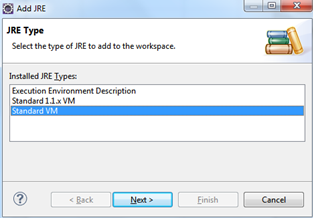
\includegraphics{figuras/anexo/selectJVM.png}
		\legend {\fontsize{10}{12}\selectfont {Fonte: Autoria Própria}.}	
	\end{subfigure}
\end{figure}


Após a seleção é preciso confirmar a ação clicando em Next, na nova janela exibida o botão Directory... permite localizar o diretório onde está a versão do JDK que será utilizada, dessa forma deve ser selecionado o diretório raiz da versão, no exemplo representado por \textit{C:/pessoal/java/jdk1.5.0\_22}, conforme visto na figura \ref{figura:anexo2};

\begin{figure}[H]
	\centering
	\caption*{\textbf{Adicionar nova JRE na IDE.}}
	\label{figura:anexo2}
	\begin{subfigure}[H]{\textwidth}
		\centering
		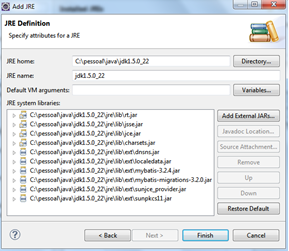
\includegraphics{figuras/anexo/addJRE.png}
		\legend {\fontsize{10}{12}\selectfont {Fonte: Autoria Própria}.}	
	\end{subfigure}
\end{figure}

A própria IDE já preenche o JRE name, caso isso não ocorra será necessário preencher este campo de preferência com o nome da versão do JDK utilizada, realizado este passo a IDE terá condições de compilar as instruções contidas no fonte.  Com isso será necessário importa o projeto no GSAN na IDE de desenvolvimento, selecionando a opção \textit{File > Import..}, abrirá um janela onde deve ser selecionando a opção \textit{General > Existing Projects into Workspace}, em seguida através do botão \textit{Browser} será possível localizar o diretório onde está o fonte do sistema GSAN, conforme ilustrado na figura \ref{figura:anexo3};

\begin{figure}[H]
	\centering
	\caption*{\textbf{Importar Sistema GSAN na IDE.}}
	\label{figura:anexo3}
	\begin{subfigure}[H]{\textwidth}
		\centering
		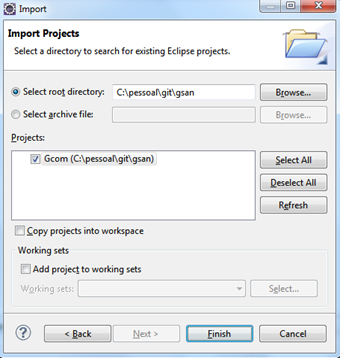
\includegraphics{figuras/anexo/importGSAN.png}
		\legend {\fontsize{10}{12}\selectfont {Fonte: Autoria Própria}.}	
	\end{subfigure}
\end{figure}


Feito isso precisa somente pressionar o botão de \textit{Finish}, para confirmar a importação do projeto para a IDE de desenvolvimento.

\chapter{Configurar variável de ambiente do servidor de aplicação Jboss}

Neste trabalho foi utilizado o projeto \textit{Open Source Jboss Community} na versão 4.0.1, compatível com as tecnologias utilizadas no GSAN, para utilizá-lo será preciso declarar uma variável de ambiente no sistema operacional, por padrão nomeado de JBOSS\_HOME contendo a localização do diretório do servidor de aplicação, no exemplo abaixo representado por \textit{C:/pessoal/jboss/jboss-4.0.1sp1}, conforme visto na figura \ref{figura:anexo4};

\begin{figure}[H]
	\centering
	\caption*{\textbf{Adicionando variável de ambiente JBOSS\_HOME.}}
	\label{figura:anexo4}
	\begin{subfigure}[H]{\textwidth}
		\centering
		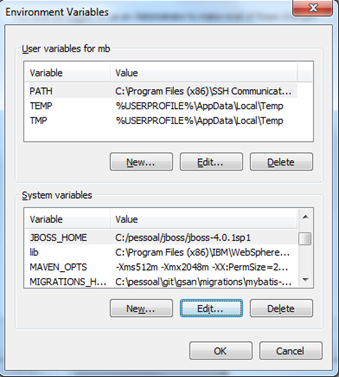
\includegraphics{figuras/anexo/var_JBOSS_HOME.png}
		\legend {\fontsize{10}{12}\selectfont {Fonte: Autoria Própria}.}	
	\end{subfigure}
\end{figure}


Após a criação desta variável de ambiente, será preciso atualizar a variável de ambiente chamada PATH que reúne as variáveis utilizadas no sistema operacional, adicionando ao final o seguinte texto \textit{\%JBOSS\_HOME\%/bin;} para que o sistema operacional consiga localizar o diretório /bin do servidor de aplicação que contém o script de inicialização do servidor chamado \textit{run.bat} para sistemas Windows e \textit{run.sh} para sistemas Unix, neste script é possível modificar os parâmetros utilizados na execução do servidor de aplicação sob a JVM para a alocação de memória assim como habilitar a utilização de técnicas de debug remoto das aplicações.


\chapter{Configuração do Fluxo da URA}
Segue abaixo a configuração do fluxo completo da URA, configurado no seguinte arquivo de configuração \textit{/etc/asterisk/extension.conf};
\\[8pt]
; Declarando o contexto de boas vindas para executar o áudio ‘inicial’ \\
; o dígito representa a rotina associada abaixo: \\
; 1 – Contexto de identificação do Cliente. \\
; 2 – Falar com o atendente. \\
\textbf{[disc-ivr-BOAS\_VINDAS] }	 \\
exten => s,1,Playback(custom/inicial)  \\
exten => 1,1,Goto(disc-ivr-IDENTIFICACAO,7001,1)  \\
exten => 2,1,Goto(FALAR\_ATENDENTE,s,1)  \\
 \\
; Declarando o contexto de identificação do cliente, executa o áudio  \\
; ‘identificacao’ e redireciona para o contexto de PESQUISAR\_CLIENTE \\
; executa o áudio ‘pronto’ e ‘numero\_ra’, soletra o numero do RA e  \\
; direciona para o Menu principal. \\
\textbf{[disc-ivr-IDENTIFICACAO]} \\
exten => 7001,1,Playback(custom/identificacao) \\
exten => 7001,2,Goto(PESQUISAR\_CLIENTE,s,1) \\
exten => 7001,3,Playback(custom/pronto) \\
exten => 7001,4,Playback(custom/numero\_ra) \\
exten => 7001,5,SayDigits(\${NUMERO\_RA}) \\
exten => 7001,6,Goto(disc-ivr-MENU,7002,1) \\
 \\
; Declara o context do Menu Principal, executa o áudio ‘menu’, \\
; o dígito representa a rotina associada abaixo: \\
; 1 – Serviço de 2ª via de Conta \\
; 2 – Serviço de Informar Falta de Água \\
; 3 – Serviço de Solicitar Restabelecimento da Ligação \\
; 4 – Falar com o atendente. \\
\textbf{[disc-ivr-MENU]} \\
exten => 7002,1,Playback(custom/menu) \\
exten => 1,1,Goto(disc-ivr-2VIA,7003,1) \\
exten => 2,1,Goto(disc-ivr-INFORMAR\_FALTA\_AGUA,7004,1) \\
exten => 3,1,Goto(disc-ivr-SOLICITAR\_RESTABELECIMENTO,7005,1) \\
exten => 4,1,Goto(FALAR\_ATENDENTE,s,1) \\
 \\
; Declarando o contexto de 2ª via, executa o aúdio ‘2via’ \\
; redireciona para o contexto de obter segunda via e \\
; desliga a ligação. \\
\textbf{[disc-ivr-2VIA]} \\
exten => 7003,1,Playback(custom/2via) \\
exten => 7003,2,Goto(OBTER\_SEGUNDA\_VIA,s,1) \\
exten => 7003,3,Hangup() \\
 \\
; Declarando o contexto disc-ivr-INFORMAR\_FALTA\_AGUA \\
; Executa o áudio ‘falta\_agua\_abrir\_chamado’  \\
; Redireciona para o contexto INFORMAR\_FALTA\_AGUA \\
; Executa o áudio ‘sucesso’ \\
; Desliga a ligação \\
\textbf{[disc-ivr-INFORMAR\_FALTA\_AGUA]} \\
exten => 7004,1,Playback(custom/falta\_agua\_abrir\_chamado) \\
exten => 7004,2,Goto(INFORMAR\_FALTA\_AGUA,s,1) \\
exten => 7004,3,Playback(custom/sucesso) \\
exten => 7004,4,Hangup() \\
 \\
; Declarando o contexto disc-ivr-SOLICITAR\_RESTABELECIMENTO \\
; Executa o áudio ‘restabelecimento’  \\
; Redireciona para o contexto SOLICITAR\_RESTABELECIMENTO \\
; Executa o áudio ‘sucesso’ \\
; Desliga a ligação \\
\textbf{[disc-ivr-SOLICITAR\_RESTABELECIMENTO]} \\
exten => 7005,1,Playback(custom/restabelecimento) \\
exten => 7005,2,Goto(SOLICITAR\_RESTABELECIMENTO,s,1) \\
exten => 7005,3,Playback(custom/sucesso) \\
exten => 7005,4,Hangup() \\
 \\
; Declarando o contexto ‘PESQUISAR\_CLIENTE’ \\
; Atende a ligação \\
; Executa o áudio ‘beep’ \\
; Defini o tempo limite de espera entre a discagem dos dígitos \\
; Defini o tempo limite de espera do primeiro dígito \\
; Ler os digitos informados \\
; Cria a variável ‘CLIENTE\_IMOVEL’ recebendo os digitos. \\
; Executa uma requisição Agi para ‘192.168.43.2/pesquisar.imovel.cliente.agi’ \\
; Exibe o ID\_IMOVEL \\
; Verifica a situação da requisição realizada \\
; Caso seja ‘SUCESSO’ redireciona para o contexto disc-ivr-IDENTIFICACAO \\
; Caso seja diferente de sucesso redireciona para FALAR\_ATENDENTE \\
\textbf{[PESQUISAR\_CLIENTE]} \\
exten => s,1,Answer() \\
exten => s,n,PlayBack(beep) \\
exten => s,n,Set(TIMEOUT(digit)=3)  \\
exten => s,n,Set(TIMEOUT(response)=7)  \\
exten => s,n,Read(NUMERO) ; LER OS DIGITOS \\
exten => s,n,Set(CLIENTE\_IMOVEL=\${NUMERO}) \\
exten => s,n,Agi(agi://192.168.43.2/pesquisar.imovel.cliente.agi) \\
exten => s,n,NoOp(\${ID\_IMOVEL}) \\
exten => s,n,GotoIf(\$["\${SITUACAO}" == "SUCESSO"]?ok:falha) \\
exten => s,n(ok),Goto(disc-ivr-IDENTIFICACAO,7001,3) \\
exten => s,n(falha),Goto(FALAR\_ATENDENTE,s,1) \\
 \\
; Declarando o contexto ‘OBTER\_SEGUNDA\_VIA’ \\
; Atende a ligação \\
; Executa uma requisição Agi para ‘192.168.43.2/segunda.via.agi’ \\
; Printa o ‘ID\_IMOVEL’ \\
; Verifica a situação da requisição realizada \\
; Caso seja ‘SUCESSO’ redireciona para o contexto ‘disc-ivr-2VIA’ \\
; Caso seja diferente de sucesso redireciona para ‘FALAR\_ATENDENTE’ \\
\textbf{[OBTER\_SEGUNDA\_VIA]} \\
exten => s,1,Answer() \\
exten => s,n,Agi(agi://192.168.43.2/segunda.via.agi) \\
exten => s,n,NoOp(\${ID\_IMOVEL}) \\
exten => s,n,GotoIf(\$["\${SITUACAO}" == "SUCESSO"]?ok:falha) \\
exten => s,n(ok),Goto(disc-ivr-2VIA,7003,3) \\
exten => s,n(falha),Goto(FALAR\_ATENDENTE,s,1) \\
\\
; Declarando o contexto ‘INFORMAR\_FALTA\_AGUA’ \\
; Atende a ligação \\
; Executa uma requisição Agi para ‘192.168.43.2/falta.agua.agi’ \\
; Verifica a situação da requisição realizada \\
; Caso seja ‘SUCESSO’ redireciona para o contexto \\
; ‘disc-ivr-NFORMAR\_FALTA\_AGUA’ \\
; Caso seja diferente de sucesso redireciona para ‘FALAR\_ATENDENTE’ \\
\textbf{[INFORMAR\_FALTA\_AGUA]} \\
exten => s,1,Answer() \\
exten => s,n,Agi(agi://192.168.43.2/falta.agua.agi) \\
exten => s,n,GotoIf(\$["\${SITUACAO}" == "SUCESSO"]?ok:falha) \\
exten => s,n(ok),Goto(disc-ivr-INFORMAR\_FALTA\_AGUA,7004,3) \\
exten => s,n(falha),Goto(FALAR\_ATENDENTE,s,1) \\
 \\
; Declarando o contexto ‘SOLICITAR\_RESTABELECIMENTO’ \\
; Atende a ligação \\
; Executa uma requisição Agi para ‘192.168.43.2/restabelecimento.ligacao.agi’ \\
; Verifica a situação da requisição realizada \\
; Caso seja ‘SUCESSO’ redireciona p/ o contexto \\
; ‘disc-ivr-SOLICITAR\_RESTABELECIMENTO \\
; Caso seja diferente de sucesso redireciona para ‘FALAR\_ATENDENTE’ \\
\textbf{[SOLICITAR\_RESTABELECIMENTO]} \\
exten => s,1,Answer() \\
exten => s,n,Agi(agi://192.168.43.2/restabelecimento.ligacao.agi) \\
exten => s,n,GotoIf(\$["\${SITUACAO}" == "SUCESSO"]?ok:falha) \\
exten => s,n(ok),Goto(disc-ivr-SOLICITAR\_RESTABELECIMENTO,7005,3) \\
exten => s,n(falha),Goto(FALAR\_ATENDENTE,s,1) \\
 \\
; Declarando o contexto ‘FALAR\_ATENDENTE’ \\
; Executa o áudio ‘ligacao\_redirecionada’ \\
; Realiza uma ligação para o ‘ATENDENTE’ \\
\textbf{[FALAR\_ATENDENTE]} \\
exten => s,1,PlayBack(custom/ligacao\_redirecionada) \\
exten => s,2,Dial(SIP/ATENDENTE) \\


\chapter{Registros de Atendimentos Gerados}

A execução dos cenários de testes resultaram na criação dos seguintes Registros de Atendimentos no sistema GSAN,
a seguir pode ser consultado o detalhamento sobre os Registros de Atendimentos gerados para o serviço Informar Falta de Água.
\begin{figure}[H]
	\centering
	\caption*{\textbf{Informar Falta de Água - Cenário 1 Detalhado.}}
	\begin{subfigure}[H]{\textwidth}
		\centering
		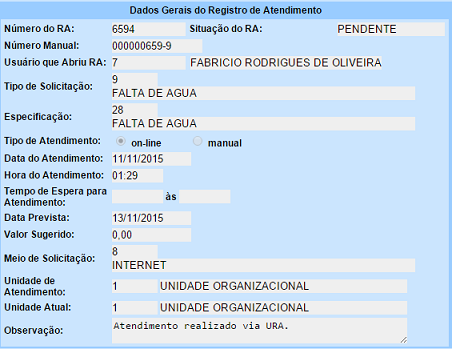
\includegraphics{figuras/anexo/falta_agua/detalhe_1.png}
		\legend {\fontsize{10}{12}\selectfont {Fonte: Autoria Própria}.}	
	\end{subfigure}
\end{figure}

\begin{figure}[H]
	\centering
	\caption*{\textbf{Informar Falta de Água - Cenário 2 Detalhado.}}
	\begin{subfigure}[H]{\textwidth}
		\centering
		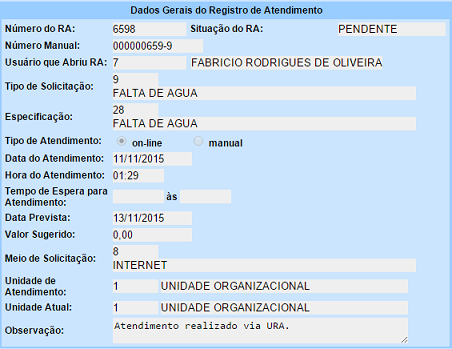
\includegraphics{figuras/anexo/falta_agua/detalhe_2.png}
		\legend {\fontsize{10}{12}\selectfont {Fonte: Autoria Própria}.}	
	\end{subfigure}
\end{figure}

\begin{figure}[H]
	\centering
	\caption*{\textbf{Informar Falta de Água - Cenário 3 Detalhado.}}
	\begin{subfigure}[H]{\textwidth}
		\centering
		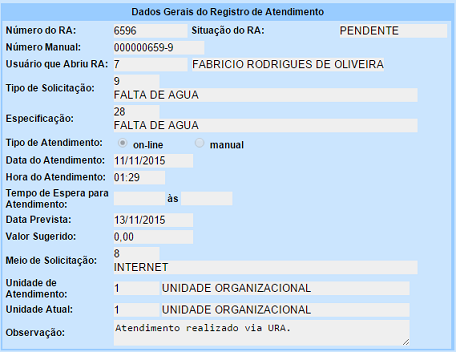
\includegraphics{figuras/anexo/falta_agua/detalhe_3.png}
		\legend {\fontsize{10}{12}\selectfont {Fonte: Autoria Própria}.}	
	\end{subfigure}
\end{figure}



A seguir pode ser consultado os registros de atendimentos abertos pela execução da suíte de testes automatizados para o serviço Solicitar Restabelecimento da Ligação de Água;

\begin{figure}[H]
	\centering
	\caption*{\textbf{Solicitar Restabelecimento da Ligação de Água - Cenário 1 Detalhado.}}
	\begin{subfigure}[H]{\textwidth}
		\centering
		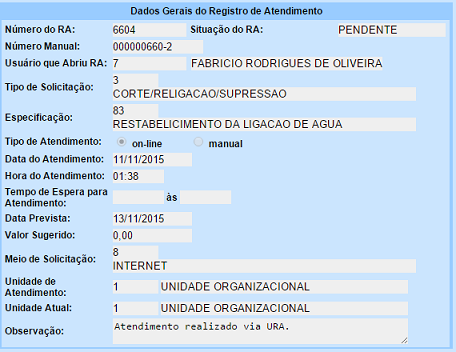
\includegraphics{figuras/anexo/restabelecer/detalhe_1.png}
		\legend {\fontsize{10}{12}\selectfont {Fonte: Autoria Própria}.}	
	\end{subfigure}
\end{figure}

\begin{figure}[H]
	\centering
	\caption*{\textbf{Solicitar Restabelecimento da Ligação de Água - Cenário 2 Detalhado.}}
	\begin{subfigure}[H]{\textwidth}
		\centering
		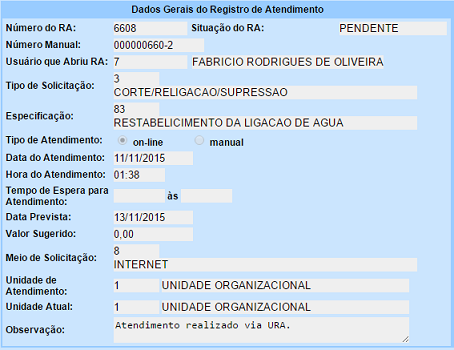
\includegraphics{figuras/anexo/restabelecer/detalhe_2.png}
		\legend {\fontsize{10}{12}\selectfont {Fonte: Autoria Própria}.}	
	\end{subfigure}
\end{figure}

\begin{figure}[H]
	\centering
	\caption*{\textbf{Solicitar Restabelecimento da Ligação de Água - Cenário 3 Detalhado.}}
	\begin{subfigure}[H]{\textwidth}
		\centering
		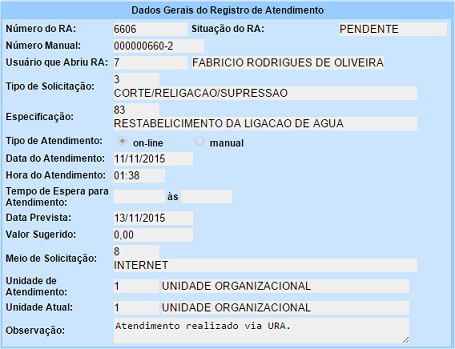
\includegraphics{figuras/anexo/restabelecer/detalhe_3.png}
		\legend {\fontsize{10}{12}\selectfont {Fonte: Autoria Própria}.}	
	\end{subfigure}
\end{figure}


\end{apendicesenv}



